\documentclass{ctexart}
\usepackage{graphicx}
\usepackage{amsmath}
\usepackage{xcolor}
\usepackage{listings}
\definecolor{mygreen}{rgb}{0,0.6,0}
\definecolor{mygrey}{rgb}{0.5,0.5,0.5}
\definecolor{mymauve}{rgb}{0.58,0,0.82}
\lstset{%
	backgroundcolor=\color{white},   % choose the background color
	basicstyle=\footnotesize\ttfamily,        % size of fonts used for the code
	columns=fullflexible,
	breaklines=true,                 % automatic line breaking only at whitespace
	captionpos=b,                    % sets the caption-position to bottom
	tabsize=4,
	commentstyle=\color{mygrey},   % comment style
	escapeinside={\%*}{*)},          % if you want to add LaTeX within your code
	keywordstyle=\color{blue},       % keyword style
	stringstyle=\color{mymauve}\ttfamily,     % string literal style
	frame=single,
	rulesepcolor=\color{red!20!green!20!blue!20},
	%identifierstyle=\color{red},
	language=python
}
\begin{document}
	
	\section{正则表达式}
	
	\begin{lstlisting}[language=python]
	#导入re包
	import re
	
	#function to check whether the pattern p can be found somewhere inside the string s.
	#re.search(p, s) 
	
	# $这个符号用于找到以ed结尾的词
	[w for w in wordlist if re.search('ed$', w)]
	#['abaissed', 'abandoned', 'abased', 'abashed', 'abatised', 'abed', 'aborted', ...]
	
	#通配符.指代单一字符
	[w for w in wordlist if re.search('^..j..t..$', w)]
	#['abjectly', 'adjuster', 'dejected', 'dejectly', 'injector', 'majestic', ...]
	\end{lstlisting}
	
	the ? symbol specifies that the previous character is optional. Thus «\^e-?mail\$» will match both email and e-mail. 
	
	\begin{lstlisting}
	#方括号中间的字母表示寻找的字符可以是任意其中之一
	[w for w in wordlist if re.search('^[ghi][mno][jlk][def]$', w)]
	#['gold', 'golf', 'hold', 'hole']
	
	# +号表示可以重复前面的字符或方括号中的字母
	>>> [w for w in chat_words if re.search('^m+i+n+e+$', w)]
	# ['miiiiiiiiiiiiinnnnnnnnnnneeeeeeeeee', 'miiiiiinnnnnnnnnneeeeeeee', 'mine',	'mmmmmmmmiiiiiiiiinnnnnnnnneeeeeeee']
	>>> [w for w in chat_words if re.search('^[ha]+$', w)]
	# ['a', 'aaaaaaaaaaaaaaaaa', 'aaahhhh', 'ah', 'ahah', 'ahahah', 'ahh',	'ahhahahaha', 'ahhh', 'ahhhh', 'ahhhhhh', 'ahhhhhhhhhhhhhh', 'h', 'ha', 'haaa',	'hah', 'haha', 'hahaaa', 'hahah', 'hahaha', 'hahahaa', 'hahahah', 'hahahaha', ...]
	
	\end{lstlisting}
	
	It should be clear that + simply means "one or more instances of the preceding item", which could be an individual character like m, a set like [fed] or a range like [d-f]. Now let's replace + with *, which means "zero or more instances of the preceding item". The regular expression «\^\ m*i*n*e*\$» will match everything that we found using «\^\ m+i+n+e+\$», but also words where some of the letters don't appear at all, e.g. me, min, and mmmmm. Note that the + and * symbols are sometimes referred to as Kleene closures, or simply closures.
	
	字符 \^\ 表示以之后的字符开头的,此外还有另外一种用法,就是在方括号的开头,比如«[\^\ aeiouAEIOU]» 就是找不是元音的字母
	
	\begin{lstlisting}
	>>> wsj = sorted(set(nltk.corpus.treebank.words()))
	>>> [w for w in wsj if re.search('^[0-9]+\.[0-9]+$', w)]
	#['0.0085', '0.05', '0.1', '0.16', '0.2', '0.25', '0.28', '0.3', '0.4', '0.5','0.50', '0.54', '0.56', '0.60', '0.7', '0.82', '0.84', '0.9', '0.95', '0.99',	'1.01', '1.1', '1.125', '1.14', '1.1650', '1.17', '1.18', '1.19', '1.2', ...]
	>>> [w for w in wsj if re.search('^[A-Z]+\$$', w)]
	#['C$', 'US$']
	>>> [w for w in wsj if re.search('^[0-9]{4}$', w)]
	#['1614', '1637', '1787', '1901', '1903', '1917', '1925', '1929', '1933', ...]
	>>> [w for w in wsj if re.search('^[0-9]+-[a-z]{3,5}$', w)]
	#['10-day', '10-lap', '10-year', '100-share', '12-point', '12-year', ...]
	>>> [w for w in wsj if re.search('^[a-z]{5,}-[a-z]{2,3}-[a-z]{,6}$', w)]
	#['black-and-white', 'bread-and-butter', 'father-in-law', 'machine-gun-toting',	'savings-and-loan']
	>>> [w for w in wsj if re.search('(ed|ing)$', w)]
	#['62%-owned', 'Absorbed', 'According', 'Adopting', 'Advanced', 'Advancing', ...]
	\end{lstlisting}
	
	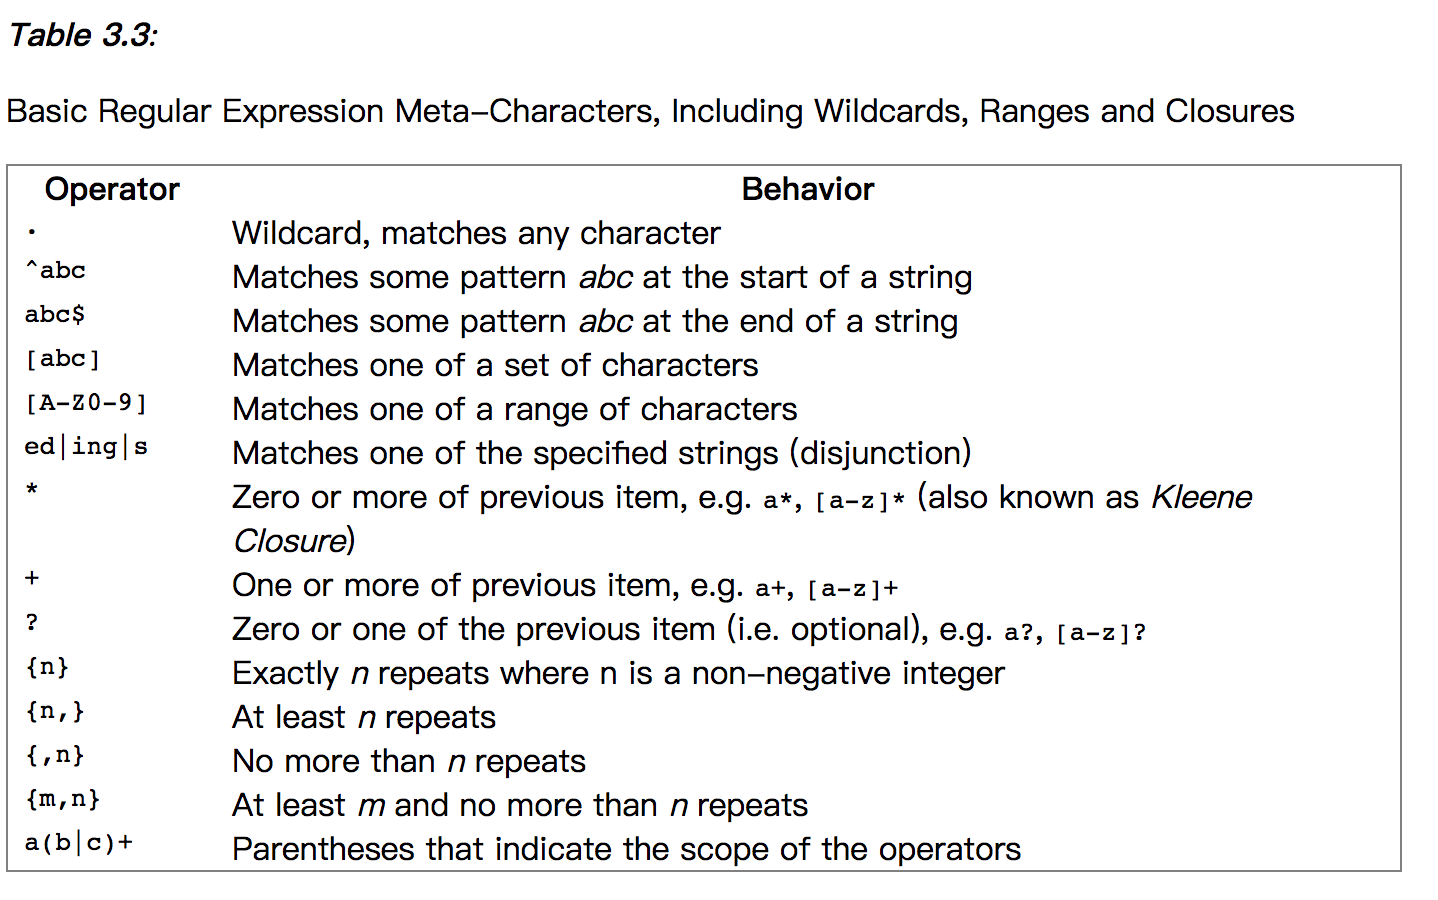
\includegraphics[width=0.8\linewidth]{pic/basic_reg_exp}
	
\end{document}